\chapter{Our Algorithm}
We consider only those cases where all the dependence distances are positive. The algorithm can then be easily extended when all dependence distances are negative for a particular loop nest.
\section{Notation}
For a nested loop, the vector of loop index for each nest is called as an iteration point. For example, consider a doubly nested loop with outer loop index i and inner loop index j. Then iteration point a = (2, 3) means that at this point, i = 2 and j = 3. Also $a_1 = 2$, $a_2 = 3.$ \\

Iteration point a is said to dominate iteration point b if\\
 $ \forall k,  a_k \leq b_k$ \\
We denote it by $a \preceq b$.\\
This creates a partial order on the set of iteration points.\\

We denote a partition by two sets of points, set A and set B, belonging to the iteration space. This partition is represented by P(A,B). \\

P(A,B) is the set of all iteration points that are dominated by at least one iteration point in set A and are not dominated by any iteration point from set B \\
$P(A,B) = \{x | ( \exists a \in A, a \preceq x) and (\forall b \in B, not(b \preceq x))\}$ \\

Thus if we have sets $A_0, A_1, ... A_k$ then we have k partitions: \\
$P(A_0,A_1), P(A_1, A_2), P(A_2, A_3), ... , P(A_{k-1}, A_k)$. \\

\subsection{Example}

For the example in figure~\ref{fig:partition_eg}, the sets are as given below: \\
$A_0 = \{(0,0)\}$ \\
$A_1 = \{(1,4), (2,2), (3,1)\}$ \\
$A_2 = \{(2,8), (3,6), (4,4), (5,3), (6,2)\}$ \\
$A_3 = \{(5,8), (6,6), (7,5), (8,4), (9,3)\}$ \\
$A_4 = \{(8,8), (9,7)\}$ \\
$A_5 = \{\}$ \\

\begin{figure}
\caption{Partitions by our algorithm}
\label{fig:partition_eg}
\centering 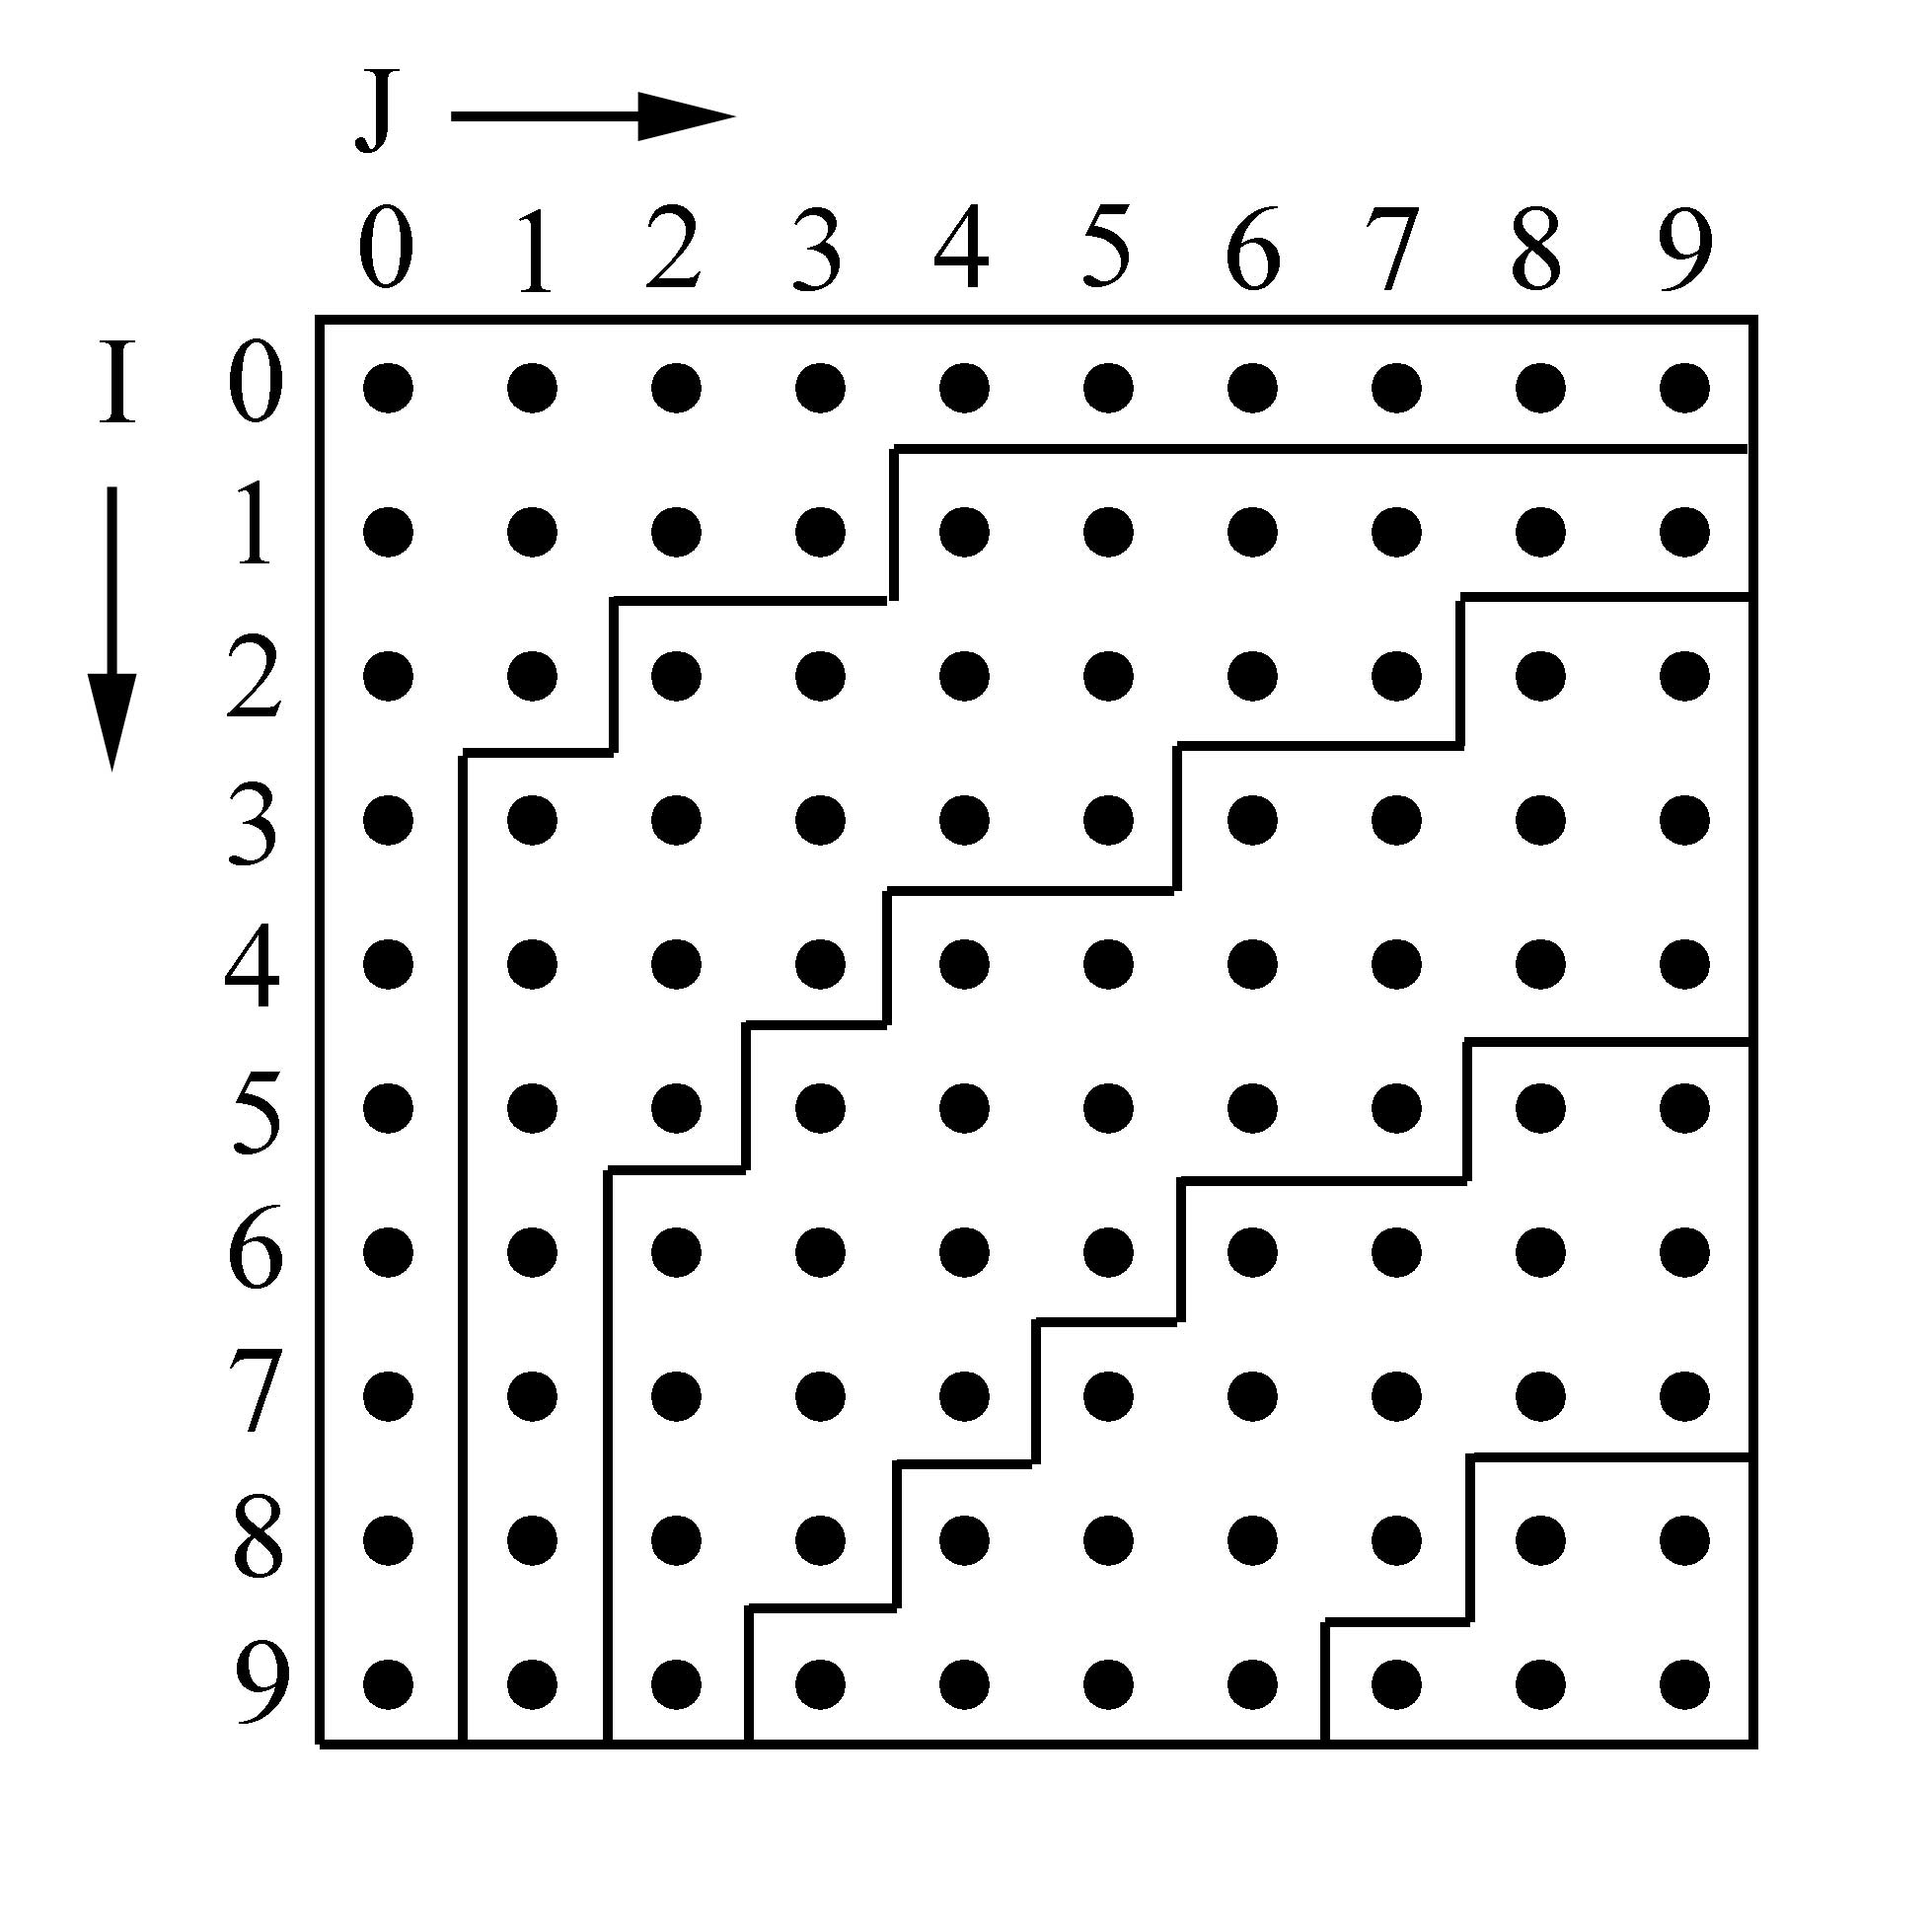
\includegraphics[width=0.5\textwidth]{Figures/fig2.jpg}
\end{figure}

%\ref{append:labelforappendix}

\section{Algorithm to generate the sets of points}

We give an iterative algorithm in which, given a set of points, it generates the next set.
Let the sets be called $A_0, A_1, .. ,A_k$ \\

Consider the set of all the dependence distances of the loop. 
Create a minimal set of dependence distances by removing any dependence distance that is dominated by another dependence distance in the set.
Thus in the minimal set, no dependence distance dominates any other dependence distance.
Call this set D. \\

\noindent
$A_0 = \{(0,0,..,0)\}$ /* Vector containing as many 0s as the total loop nest. First element corresponds to outermost loop and so on. */ \\
$iter = 0$ \\
while($A_{iter}$ is not empty) \{ \\
\indent	iter++ \\
\indent	$B = \{\}$ \\
\indent	$ \forall a \in A_{iter-1}, \forall d \in D$, insert a+d in B if a+d lies inside the loop bounds\\
\indent	Create a minimal set of B, by removing an iteration point from B if there exists another iteration point dominating it.\\
\indent	Thus in the final set obtained no iteration point dominates another point.\\
\indent	Set $A_{iter}$ as this minimal set obtained\\
\} \\

\subsection{Example}

\noindent For example consider the following code: \\
DO I = 0 to 9 \\
\indent DO J = 0 to 9 \\
\indent \indent A[I+1, J+4] = B[I, J] \\
\indent \indent C[I+2, J+2] = A[I, J] \\
\indent \indent B[I+3, J+1] = C[I, J] \\
\indent ENDO \\
ENDO \\

\noindent In this case, \\
$D = \{(1,4), (2,2), (3,1)\}$ \\
The above algorithm apllied to this example is shown in table~\ref{table:iterations}. \\
The partitions generated are depicted in figure~\ref{fig:partition_eg}. \\

\begin{table}
\caption {Iterations of the algorithm applied to example}
\label{table:iterations}
\begin{tabular}{|c| L{5.75cm} | L{5.75cm} | }

\hline

\bf iter &
\bf B &
\bf $A_{iter}$ \\ \hline

\bf 0 &
- &
$\{(0,0)\}$ \\ \hline

\bf 1 &
$\{(1,4), (2,2), (3,1)\}$ &
$\{((1,4), (2,2), (3,1)\}$ \\ \hline

\bf 2 &
$\{(2,8), (3,6), (4,5), (3,6), (4,4),$ $(5,3), (4,5), (5,3), (6,2)\}$ &
$\{(2,8), (3,6), (4,4), (5,3), (6,2)\}$ \\ \hline

\bf 3 &
$\{(5,9), (5,8), (6,7), (5,8), (6,6),$ $(7,5), (6,7), (7,5), (8,4), (7,6),$ $(8,4), (9,3)\}$ &
$\{(5,8), (6,6), (7,5), (8,4), (9,3)\}$ \\ \hline

\bf 4 &
$\{(8,9), (8,8), (9,7), (8,9), (9,7),$ $(9,8)\}$ &
$\{(8,8), (9,7)\}$ \\ \hline

\bf 5 &
$\{\}$ &
$\{\}$ \\ \hline

\end{tabular}
\end{table}
